\section{La situación y el relieve de Europa}

Europa es un continente pequeño por su extensión. Está situado en el hemisferio norte de la Tierra. Está entre los océanos Glacial Ártico y Atlántico, y entre los continentes de Asia y África. Sus límites son el océano Glacial Ártico, al norte; el mar Mediterráneo, al sur; los montes Urales, el mar Caspio, el Cáucaso y el mar Negro, al este; y el océano Atlántico, al oeste.

\subsection{El relieve}

\subsubsection{El relieve de interior: llanuras, montañas antiguas y montañas jóvenes}

\begin{itemize}
    \item Las \textbf{llanuras} se encuentran en el centro del continente y destaca la Gran Llanura Europea.
    \item Las \textbf{mesetas} y las \textbf{montañas antiguas} poco elevadas y de formas redondeadas se encuentran en el norte y en el centro del continente. Destacan el macizo Central francés, los Montes Escandinavos y los montes Urales.
    \item Las \textbf{montañas jóvenes} de gran altura se localizan en el sur del continente. Las más importantes son los Pirineos, los Alpes, los Apeninos, los Cárpatos y el Cáucaso.
\end{itemize}

\subsubsection{El relieve de costa}

Las costas de Europa son muy recortadas, debido a que abundan penínsulas, como la ibérica, la itálica…; cabos, como Norte, Fisterra...; y golfos, como Génova, Bizkaia, Botnia... También pertenecen al continente europeo muchas islas:
\begin{itemize}
    \item En el océano Atlántico se localizan las islas de Islandia, Irlanda, Gran Bretaña, Azores, Madeira, el archipiélago de Canarias, etc.
    \item En el mar Mediterráneo se encuentran las islas de Córcega, Cerdeña, Sicilia, Malta, Creta y Chipre, el archipiélago de Baleares, etc.
\end{itemize}

\subsection{La modificación del relieve}

El relieve, tanto de interior como de costa, sufre modificaciones debido a causas internas y externas. Las \textbf{causas internas} (Figura \ref{fig:causas-internas}) provocan el levantamiento, el hundimiento o el desplazamiento del terreno. En ocasiones, se manifiestan de forma violenta produciendo catástrofes naturales. Destacan los terremotos, los tsunamis, o terremotos submarinos, y los volcanes. Las \textbf{causas externas} (Figura \ref{fig:causas-externas}) desgastan el relieve, transportan los materiales y los depositan en ciertas áreas. Los principales agentes externos son la atmósfera, el agua y los seres vivos.

\begin{figure}[!ht]
    \centering
    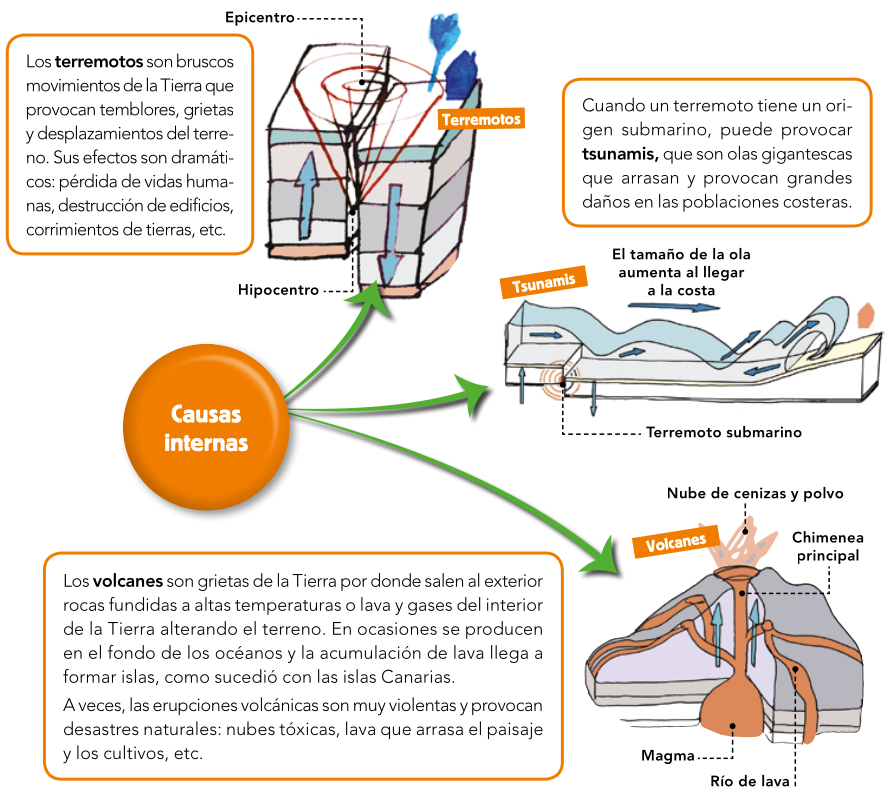
\includegraphics[width=0.7\linewidth]{Tema2/05_causas_internas.png}
    \caption{Causas internas de la modificación del relieve}
    \label{fig:causas-internas}
\end{figure}

\begin{figure}[!ht]
    \centering
    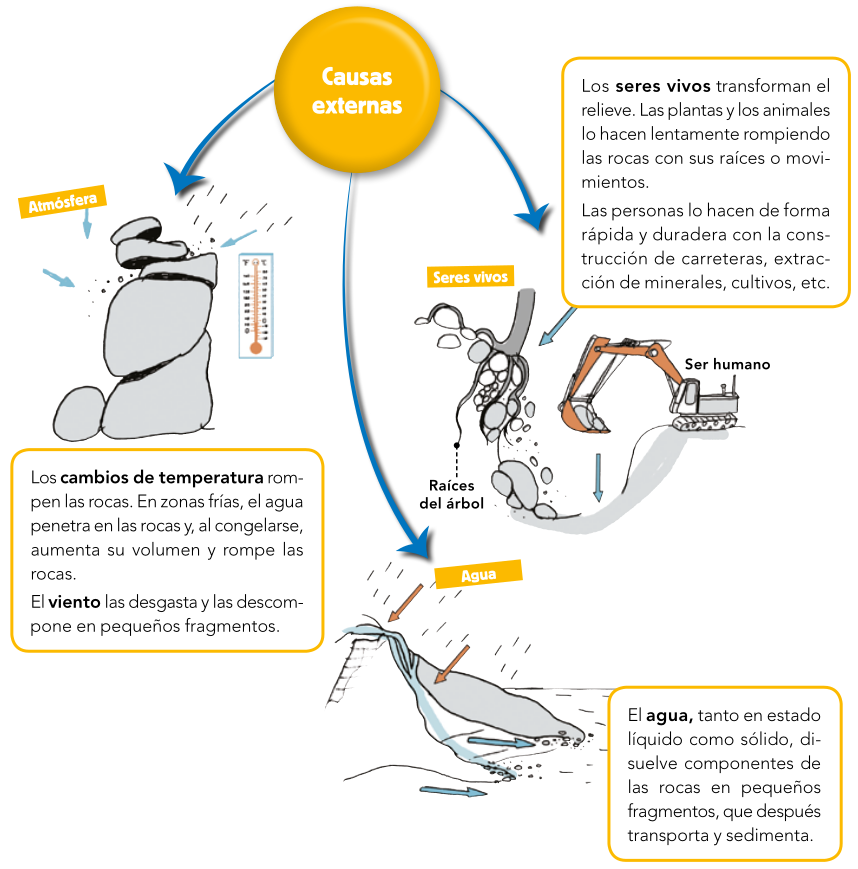
\includegraphics[width=0.7\linewidth]{Tema2/06_causas_externas.png}
    \caption{Causas externas de la modificación del relieve}
    \label{fig:causas-externas}
\end{figure}